\subsection{X-Axis: Horizontal Duplication}
\label{sec:x-axis}

The x-axis of the cube of the scalability is concerned with the horizontal
duplication and cloning of services and data with absolutely no bias, running
each identical copy of the system on a different server. Usually, the work is
distributed by a load balancer.

Reasoning on the x-axis is typically easy and the implementation can be fast,
but the data sets have to be replicated in their entirety which increases
operational costs.

\subsubsection{An example: Web server replication}
In order to better understand the concept, we bring an example of a common
architecture which scales on this axis. Let's consider a small e-commerce
business that runs its website on a single server on top of a single machine.
This website is becoming increasingly popular and suddenly, it has to face the
explosive growth of HTTP requests. If this trend continues, the website cannot
scale-up for along time.

After a technical advice, the owner of the business decides to take Web server 
codebase and deploy an identical copy of it. To make the website work on two
different servers, she decides to use
\texttt{nginx}\footnote{\url{http://nginx.org/}}. It is an HTTP and reverse
proxy server, mail proxy server and a generic TCP/UDP proxy server. Among the
HTTP server features, it serves as load balancer. The load balancing methods
supported by \texttt{nginx} are:

\begin{itemize}
  \item round-robin, the requests are distributed in round-robin
  \item least-connected, the next request is assigned to the server with the
  least number of active connections
  \item ip-hash, the request is assigned to a server based on the client's IP
  address
\end{itemize}

The two Web servers now work in parallel and access the same database and,
if they are \emph{stateless}, the owner can choose any of the load 
balancing methods offered by the load balancer. Statelessness is an important
property in this scenario, it avoids dependency between requests, that is the
server can process a request without needing to access the information of
another one. In the example, if the servers would not have been stateless (i.e.
stateful), one request arrived at one of the two servers could be the ones
on which another request being processing on the other server depends on, hence
without permitting to successfully fulfill the latter.


\begin{figure}
  \centering
  \begin{subfigure}[m]{.4\textwidth}
    \centering
    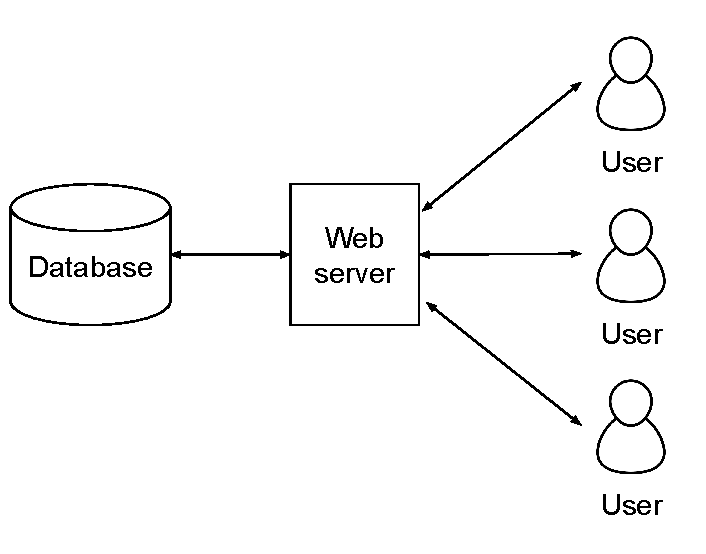
\includegraphics[height=4cm]{./res/img/webserver.pdf}
    \caption{}
    \label{fig:webserver}
  \end{subfigure}
  \hskip 3em
  \begin{subfigure}[m]{.4\textwidth}
    \centering
    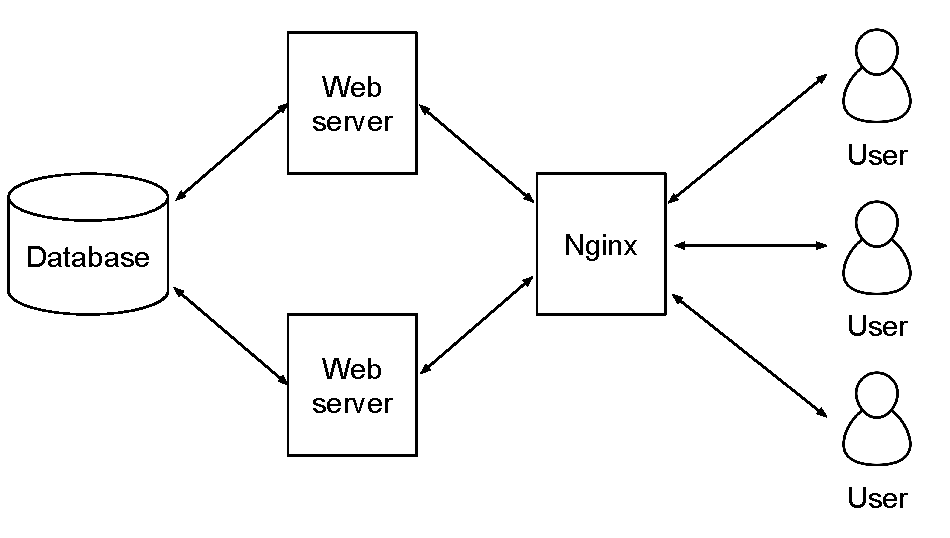
\includegraphics[height=4cm]{./res/img/webserver-nginx.pdf}
    \caption{}
    \label{fig:webserver-nginx}
  \end{subfigure}
  \caption{Web servers without (\protect\subref{fig:webserver}) and with (\protect\subref{fig:webserver-nginx}) load balancer.}
  \label{fig:webserver-scale-x}
\end{figure}

\subsubsection{State}
Let's clarify the concept of \emph{state} in order to better understand the
importance of it for scaling on the x-axis. We said that, in other words, an
application that uses state chooses the next action to be performed evaluating
the current execution condition \cite{bib:art-of-scalability}. This definition
holds for the protocols as well. A common example of stateless protocol is HTTP,
since it does not need to know anything about a previous request having all the
information needed to fulfill the current request. On the contrary, an example
of stateful application is a possible implementation of user session (which can
be done also with a stateless approach), in which a user is authorized to
request some resources only after an authentication request. In this setting,
the result of the authentication could be stored in the server making it
stateful, i.e. some requests are dependent on the authentication request.
Referring at \autoref{fig:webserver-nginx}, in the stateful implementation, the
user sessions could be stored at Web server level. In our example, the only load
balancing method which supports session persistence is \emph{ip-hash} thanks to
its ability to always redirect requests from a client to the same server except
when this server is unavailable or when the client's IP address changes. Indeed,
with \emph{round-robin} and \emph{least-connected} each request is potentially
distributed to a different server making it necessary to write stateless
servers.
% add comparison between this state and the Ethereum state

It should be clear now the role of the \emph{state} scaling on the x-axis. Once
we scale by cloning, we duplicate the data along with the service. If the state
changes, these changes should be reflected on the server which accesses that
same part of the state. This can be not a drawback at first, but it may become
an issue increasing the data size.

\subsubsection{Ethereum current state and proposals}
\label{sec:x-axis-ethereum}

In~\autoref{sec:consensus:algorithm}, we introduced the Ethereum consensus
algorithm and the PoW algorithm which is run by the miners in order to create
the next valid block. The more miners join the network (or improve the
existents), thus incrementing the global hash rate, the more difficult a state
transition become. In \autoref{sec:max-troughput}, we measure the maximal
transaction throughput in a private blockchain\footnote{See~\autoref{sec:tests}
for a detailed tests description.}. Incrementing the number of miners in the
network does not increment the transaction throughput, indeed it is almost
negatively affected. This decreasing in performance can be due to a variety of
factors like network overhead, ``unluckiness'' of the miners which affects the
mining difficulty, or perturbation in the performance of the nodes, but it is
not relevant for the purpose of the test. Another significant test we present is
described in \autoref{sec:max-throughput-high-gaslimit}. In this test we set a
gas limit high enough to not restrict the number of transactions which can be
included in a block. The results show a little increment in the transaction
throughput with regards to the previous test, but again the number of miners
does not affect the overall performance. Hence, duplicating the miners in the
network does not increment the transaction throughput making the scaling on the
x-axis absent in the current implementation. When we are talking about
duplicating, we are not assuming the nodes are running the same implementation.
Indeed, there are multiple implementations (e.g.,
geth\footnote{\url{https://github.com/ethereum/go-ethereum}},
parity\footnote{\url{https://github.com/paritytech/parity}}, etc.), that adhere
to the same protocols, therefore they are functionally equivalent.

In \autoref{sec:background}, we already pointed out that Ethereum is stateful,
thus making it difficult to scale on the x-axis. Moreover, the implementation of
the consensus layer requires that everyone validates each block propagated in
the network executing all the transactions and the EVM computations which is in
contrast with the concept of load distribution of the x-axis. Thus, the system
is limited by the performance of the single computer duplicated in the network.
Because of these issues, it is very difficult to individuate measures to scale
on this axis without loosing other fundamental characteristics, like
decentralization and trustlessness. Without these latter features, we would have
a traditional system with a central authority on which we could implement some
well know scaling solutions such as load balance among the different servers or
simply scale up.
